% Thesis!

% Two Column Format
\documentclass[11pt]{article}
%this allows us to specify sections to be single or multi column so that things like title page and table of contents are single column
\usepackage{multicol, caption}
\usepackage{verbatim}
\usepackage{listings}
\usepackage{color}
\usepackage{todonotes}

\definecolor{dkgreen}{rgb}{0,0.6,0}
\definecolor{gray}{rgb}{0.5,0.5,0.5}
\definecolor{mauve}{rgb}{0.58,0,0.82}

\lstdefinelanguage{JavaScript}{
  keywords={typeof, new, true, false, catch, function, return, null, catch, switch, var, if, in, while, do, else, case, break},
  keywordstyle=\color{blue}\bfseries,
  ndkeywords={class, export, boolean, throw, implements, import, this},
  ndkeywordstyle=\color{darkgray}\bfseries,
  identifierstyle=\color{black},
  sensitive=false,
  comment=[l]{//},
  morecomment=[s]{/*}{*/},
  commentstyle=\color{purple}\ttfamily,
  stringstyle=\color{red}\ttfamily,
  morestring=[b]',
  morestring=[b]"
}

\lstset{frame=tb,
  language=JavaScript,
  aboveskip=3mm,
  belowskip=3mm,
  showstringspaces=false,
  columns=flexible,
  basicstyle={\small\ttfamily},
  numbers=none,
  numberstyle=\tiny\color{gray},
  keywordstyle=\color{blue},
  commentstyle=\color{dkgreen},
  stringstyle=\color{mauve},
  breaklines=true,
  breakatwhitespace=true
  tabsize=3
}

\usepackage{setspace}
\usepackage{url}

\usepackage{graphicx}

%%% PAGE DIMENSIONS
\usepackage{geometry} % to change the page dimensions
\geometry{letterpaper}

\setcounter{secnumdepth}{5}

\graphicspath{ {./images/} }

\newenvironment{Figure}
  {\par\medskip\noindent\minipage{\linewidth}}
  {\endminipage\par\medskip}

\begin{document}

%%%%%%%%%%%%%%%%%%
%%% Cover Page %%%
%%%%%%%%%%%%%%%%%%

\title{\vfill A Testing Framework for Web Applications} %\vfill gives us the black space at the top of the page
\author{
By Taggart Ashby \vspace{10pt} \\
}

\maketitle

\vfill  %in combination with \newpage this forces the abstract to the bottom of the page

%%%%%%%%%%%%%%%%
%%% Abstract 
%%% VERY General overview of problem and solution in paper
%%%%%%%%%%%%%%%%
\begin{abstract}
We have brought together a number of testing tools from the web and created what we feel is a fully-featured, easy to use, testing framework for web applications.
\end{abstract}

\thispagestyle{empty} %remove page number from title page
\newpage

%end the 1 column format

%start 2 column format
% \begin{multicols}{2}
%Start numbering first page of content as page 1
\setcounter{page}{1}

%%%%%%%%%%%%%%%%%%%%
%%% Introduction/Motivation
%%% More detailed, but still general, description of problem and why we want to solve it
%%%%%%%%%%%%%%%%%%%%
\section{Introduction}
Since the advent of the internet, the web has undergone an impressive evolution from plain-text webpages to the highly stylized and functional pages that we see today. In the last four to six years there has been an explosion of new web technologies that make applications more functional: HTML5, CSS3, WebGL, Touch APIs, Geo-location, and a host of others. \cite{EvolutionOfWeb} In that same time period, the number of global internet users has grown to somewhere around 2.5 billion people. \cite{EvolutionOfWeb} The combination of these new technologies and the ever-increasing usage of the internet has led to a significant growth in the number and complexity of web applications.
Like any piece of software, these web applications require testing in order to determine their correctness and give their users the best experience possible. Unfortunately, web applications are new and there are no standard practices regarding how to test them. Their dynamic nature and network communication require a different testing toolkit than their predecessors. In addition, web applications are being produced at an incredible rate and so there's a need for rapid testing.

We can see that this is not a solved problem by looking at some of the biggest web application around. A 2011 study showed that YouTube has at least eight errors, Apple has at least seven, Microsoft at least four, and the list goes on. \cite{ErrorsInTheWild} That may seem like a incredibly small amount for such monoliths, and, honestly, it is fairly small, but those are still errors in the software that ought to be fixed.
What this all boils down to is that there needs to be a framework in place for testing these multi-layer, multi-faceted web applications that is easy to use, quick to develop on, and thorough in its coverage.

\subsection{What Has Been Done Already?}
- Info info info

\subsubsection{Why It Is Insufficient}
- No standard
- Info info info

\subsection{Problems Still Faced/Why It's So Hard}
- A lot of products to test against (browsers)
- Asynchronous shennanigans

\subsection{Contributions of This Thesis}
- Framework
- Wade through all the tools currently out there
-- Focus in, no need to have every developer check out all 10000 tools
-- Weigh options


%%%%%%%%%%%%%%%%%%
%%% Background 
%%% Information needed for reader to know what’s going on
%%% 	Server/Client Communication
%%% 	Cloud services
%%% 	Appropriate terms and definitions
%%%%%%%%%%%%%%%%%%
\section{Background}
In an effort to make the rest of the paper more understandable and to define the terms used in the remainder of the paper, it is useful to have a section pertaining to the different concepts and technologies surrounding the web.
If one is familiar with HTML5, JavaScript, and Testing concepts and statistics, it will likely be safe to skip this background section.

\subsection{Web Application Strengths}
Web applications are great for both developers and consumers. They have a number of characteristics that make them more desirable than shrink-wrap software. These attributes are versioning, availability, platform independence, and the ability to rapidly prototype.

\subsubsection{Versioning}
Web applications can be updated at any time with instant roll-out and feedback. It requires absolutely no user interaction because the web page always serves the latest resources. In comparison to something like an operating system that requires users to manually update, this feature leads to applications that can address problems quickly, roll-out security updates instantly, and incorporate consumer feedback much more quickly than any other type of software. Another perk is that users are not given a choice. This can lead to occasional customer outrage, but more often than not it's a powerful gain for both feature improvement and application security.

\subsubsection{Availability}
Web application are available anywhere there's internet. No need to install anything on a given device most of the time. Due to the ever-increasing popularity of mobile devices, most applications have both mobile and full versions of their software and so the application is ``with you'' all the time.

\subsubsection{Multi-platform}
Very similar to the availability strength, web applications are platform independent. Whether you're on your phone, tablet, laptop, or PC, the application only requires a web browser with certain functionality and in this day and age all devices come equipped with browsers that should have no problems.

\subsubsection{Rapid Prototyping}
Web applications are fantastic for rapid prototyping because of all of the strengths discussed above. An idea can be prototyped and posted on a website quickly and rapid iteration can occur without the user even necessarily noticing. There are a number of web tools that will outline where users are clicking, what features they're using, how long they're spending on a given page or step of a process, and a number of other metrics that can make iterations more directed and effective.


\subsection{Web Features}
Here I'll discuss some of the prevalent technologies that recently appeared in web applications and development. By no means is this an exhaustive list, just a sampling of the more prominent ones.

\subsubsection{HTML5}
The latest revision of HTML is HTML5 which first debuted on Firefox back in 2009. \cite{EvolutionOfWeb} HTML5 has not been officially recommended by the W3C (World Wide Web Consortium) who is the official keeper and recommender of web standards, however, there is a plan for final recommendation this year, 2014, called Plan 2014. \cite{Plan2014} What this means is that in 2014 the W3C will release a stable HTML5 Recommendation which will make HTML5 an official standard and help universalize all the separate implementations.

HTML5 brings a number of new features including: audio and video tags, the canvas element, drag-and-drop functionality, web storage, offline page support, and a number of other modern web features. A lot of HTML5's features revolve around the inclusion of multimedia in web pages and stronger graphical processing and programming.

- Talk about GeoLocation

- TIE JS PORTION INTO THIS

% \subsubsection{JavaScript}
JavaScript, though not the only scripting language with web use, is the primary language used to compliment HTML when making web applications. It is an interpreted language that is most often associated with client-side functionality, but in recent times has extended to the server-side. JavaScript is a prototype based object oriented scripting language with dynamic typing and first-class functions. Much of JavaScript's popularity stems from this dynamic nature that allows for quick, and often dirty, implementation of features in an often iterative environment.


- THIS NEEDS TO MOVE OR CHANGE SUBSECTION TO `WEB APPLICATIONS'
\subsubsection{Node.JS}
Node.JS, often called simply Node, is a JavaScript API for creating and running servers. ``Node's goal is to provide an easy way to build scalable network programs.'' \cite{Node} Node was created in 2009 and is sponsored by Joyent. Node does not use thread-based networking, instead opting for a single-threaded event loop and non-blocking I/O. Node allows developers to create and control web servers without the need for external software, such as Apache, commonly found in other sites.

Node is found in a number of popular sites including: PayPal, The New York Times, Yahoo!, Uber, LinkedIn, Microsoft Azure, and a number of others. \cite{Node}


- TIE THIS CLIENT/SERVER STUFF into Web Applications, be specific, not generic
\subsection{Client/Server Architecture}
Web applications have a user-facing client-side and a ``rear-facing'' (IS THIS THE RIGHT TERM...) server-side.

Here we'll discuss what the client-side is and does, what the server-side is and does, and how they communicate.

\subsubsection{What is the Client-side Portion?}
First, I'll address what a client is. The simple answer is: You. Your phone, computer, tablet, or other device communicating with a given website or application is the client. More specifically, the browser or service you're using to communicate with the web is the client. 

So now that the client has been clarified, what is the client-side portion of an application? The client-side portion interacts with the browser to request assets from the server and then displaying them in a human-readable way. The client-side also deals with the user interface and interactivity of a web page, e.g., the client-side displays a web form, the client fills in the information and clicks ``submit'' and the client-side packages up the data and sends it to the server-side.

Client-side programming is done in a language that the browser understands, most frequently Javascript. Though not technically programming languages, client-side programming is also done through HTML and CSS which control the look and feel of web pages.

\subsubsection{What is the Server-side Portion?}
Once again, I'll outline a server and then delve into server-side programming. A server is the entity, be it machine, person, or cloud service, that stores the information about a given web page or application. The server stores all assets, HTML pages, images, videos, databases, etc, and provides them upon request to the client. The server also handles all of the processing for interactivity, accounts, and a general number-crunching.

The server-side portion of an application, then, stores all of the assets, accounts, and structure of the entire application. The server-side authenticates users, retrieves data from databases, processes large data, and send information, be it assets or results, back to the client to display to the user.

\subsubsection{Client and Server Interactions}
The client has limited access to resources on any given web application. This access is restricted by the server. Without such restrictions in place, someone could access user databases, credit card information, order reports, etc. In addition, there would be an overwhelming amount of content for a client to parse through, even if they have no malicious intent.

Clients communicate with the Server through a request-response architecture. Clients send a request to the server, sometimes with information attached, such as a form submittal or login, and the server returns a response with either a success/failure message, or additional data.


\subsection{What is testing?}
IEEE defines software testing as ``the dynamic verification of the behavior of a program on a finite set of test cases, suitably selected from the usually infinite executions domain, against the expected behavior.'' \cite{TestingDefinition} Put a bit more simply, software testing is the process of making sure the program does what it is supposed to.

There are a number of different types of tests and testing concept, we will just focus on Unit Testing, Continuous Integration, and Acceptance Testing.

\subsubsection{Unit Testing}
Unit testing is the testing of specific functions and functionality. Generally this means the testing of individual functions but can extend to a set of functions that produce a single module of functionality. What sets Unit Testing apart from other types of testing is that tests focus on one portion of the code or system rather than interactions between modules or the entire system.

Here's a brief example:
\begin{lstlisting}
// Terribly useless code whose purpose is to eventually calculate a magic number
function addTwo (numToAddTo) {
	return numToAddTo + 2;
}

function twoTimes (numToMultiply) {
	var sum = 0;

	for (var i = 0; i < numToMultiply; i++) {
		sum = addTwo(sum);
	}

	return sum;
}

.... // More functions

function calculateMagicNumberPartOne (startingNum) {
	var foo = 3 + addTwo(startingNum);

	return twoTimes(foo);
}

... // More functions

function calculateMagicNumber (startingNum) {
	var numSoFar = calculateMagicNumberPartOne(startingNum);

	numSoFar = calculateMagicNumberPartTwo(numSoFar);
	numSoFar = calculateMagicNumberPartThree(numSoFar);
	... // More calculateMagicNumberPart(s)

	return numSoFar;
}

function testAddTwo () ... // Unit Test
function testTwoTimes () ... // Unit Test
function testCalculateMagicNumberPartOne () ... // Still a Unit Test, just a whole module of functionality

function testCalculateMagicNumber () ... // NOT a Unit Test because it's testing the whole system
\end{lstlisting}

\subsubsection{Continuous Integration}
Continuous Integration (CI), in the context of testing, also known as Continuous Testing, is the term for a piece of software or service that continually runs tests on your code as you develop. The purpose of this is to make sure that new code is not breaking old tests and that new code is passing any tests you've written for it prior to writing it. This is invaluable feedback because you can see if you're making progress in the right direction as you write code, as opposed to a situation in which you finish coding and find out you made a bad assumption or decision early on. 

One of the most important aspects of a good piece of CI software is that it is automatic. There should be no need for a developer to do anything besides ``turn it on'' and start coding. As soon as a tool, CI or otherwise, requires more than one or two interactions to run, it becomes more of a nuisance and less of an asset.

\subsubsection{Acceptance Testing}
Acceptance testing is testing to confirm that your product meets a certain specification. Often in the terms of software this is making sure that your software meets an SRS (Software Requirements Specification) or a customer's outlined expectations. Often this testing is performed by the user of the software or that customer that ordered the software, rather than the developers.

\subsubsection{Testing Statistics}
It is widely accepted that the earlier a developer detects a defect, the easier it is to fix that defect. A famous book, ``Code Complete'' by Steve McConnell \cite{DefectPic}, includes the following figure, showing this statistic on a rough graph.

\begin{Figure}
	\centering
	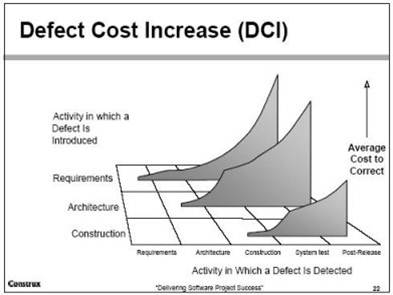
\includegraphics[width=0.75\linewidth]{defectcost.jpg} 
	\captionof{figure}{\cite{DefectPic}}
\end{Figure}

% - CONSIDER REMOVING ALTOGETHER
% \subsubsection{Why Testing is Important}
% I'm consistently surprised by how few people take testing seriously when it comes to non-trivial applications. Many developers will leave testing to their users, i.e., wait for users to have problems and report them before developers will fix them. This is an issue for a number of reasons, a few of which are: frustrated customers are unlikely to continue using a buggy product and are dissuaded from buying future products from the same developer, certain bugs can be security loopholes that may allow users access to information they shouldn't have, in the worst cases a bug may cause damage to a person or property and the developers would be on the hook.


%%%%%%%%%%%%%%%%%%%%%%%%%
%%% Product 
%%% User Manual
%%% 	Tools (programs, IDEs, scripts)
%%% 	Setup instructions
%%% 	Usage
%%%%%%%%%%%%%%%%%%%%%%%%%
\section{Product}


%%%%%%%%%%%%%%%%%%%%%%
%%% Implementation 
%%% 	Why I chose the tools I chose
%%% 	Scripts written to help out 
%%%%%%%%%%%%%%%%%%%%%%
\section{Implementation}


\section{Sample App and Testing Frameworks}

\subsection{Assumptions and Requirements}
In order to more thoroughly vet the many testing frameworks we came across, we had a number of assumptions about the projects we'd be looking at and requirements for those framework.
- Node.js server because it's JS, so it's testable.
- Something to do unit testing
- Something to do continuous integration

\subsection{Sample ToDo App}
In order to test out the various frameworks that we found online, we needed a small application with some functionality, but without the inherent complexity that was going to come with our evaluation application. After some searching, I decided upon a Todo application made with Express.js, Node.js, and MongoDB. \cite{ToDoAppHomePage} This application was selected because it included Node.js and had enough functionality that tests wouldn't be completely trivial while also not being overwhelming.
One of the challenges in testing that I quickly came across was the asynchronous nature of the MongoDB calls that were made in the sample app. Because of this headache, I will be discussing how the following frameworks deal with asynchronous test support as JavaScript is inherently asynchronous.

\subsection{Unit Testing Frameworks}
The following frameworks are reviewed in chronological order of my evaluation. As such, comparisons will generally only be drawn between a framework and its predecessors in paper order. After all of the frameworks are outlined and evaluated, a longer section regarding the final decision will be made where comparisons will be drawn between all of them. 

\subsubsection{Jasmine \cite{Jasmine}}
The first of the unit testing frameworks that I looked at was Jasmine, a Behavior Driven Development (BDD) testing framework. BDD is based on Test Driven Development and adds some simplifications and patterns that attempt to bring both developers and businessmen into the software testing process. The idea behind Behavior Driven Development is that input from non-technical stakeholders as well as technical stakeholders can come together so that everyone understands what the project should do.

This relates to Jasmine is the way that you write Jasmine tests. The idea behind jasmine tests is that they read, as much as possible, like english sentences. As an example, the following is a valid Jasmine test:
\begin{lstlisting}
describe("Arithmetic Test", function () {
  it("should be able to compute the addition of two numbers", function () {
    expect(1 + 2).toEqual(3);
  });

  it("should be able to subtract numbers", function () {
    var theAnswer = 10;

    expect(12 - 2).toEqual(theAnswer);
  });
});
\end{lstlisting}
The ``describe'' statement creates a test suite to collect related tests under. Each ``it'' statement is generally one test with some number of ``expect'' statements. It may not be particularly pretty, but the above code is quite readable even to someone with no coding experience.

The default Jasmine package had some ineptitudes in dealing with Node.js but there was a package available through npm called jasmine-node \cite{JasmineNode} that gave jasmine access to the node package and functions. 

Asynchronous testing using Jasmine was a bit of a chore, but there is support built in. This support comes in the form of a three-set function progression. The first function, ``runs(function () \{ .... \})'', runs the asynchronous code. The second function, ``waitsFor(function () \{ ... \})'', polls a flag that is set by the first function when it completes. Finally, the third function, another ``runs(...)'', houses the assertions to determine if the code ran properly or not. This method requires a fairly substantial amount of typing as well as complicated function chains when more than one asynchronous call is required.

NO WEB PAGE TESTING SO FAR

\paragraph{Pros}

\paragraph{Cons}

\subsubsection{Mocha \cite{Mocha}}
Mocha is another BDD testing framework that is almost identical to Jasmine. Unlike Jasmine, however, Mocha is not completely self-contained and requires an additional assertion library of one's choosing. I will outline my choice of Chai.js below.

Mocha also uses the ``describe -> it(\"should...\" '' pattern to create tests. There is no standard for writing expectation though, as each assertion library is likely to be slightly different.

Mocha's approach to asynchronous testing is quite a bit more straightforward than Jasmine's. In your ``it(...)'' anonymous function you pass an additional parameter called ``done'' which you then call when you know the asynchronous call has finished. This required me to edit the code I was testing to make all the async calls accept an additional callback, but it was a very small price to pay for extended testability. An example asynchronous test would look like this:
\begin{lstlisting}
describe("Asynch Mocha Test", function () {
  it("look like this", function (done) {
    myAsyncCall(param1, param2, function () {
      // This callback expected to run when async returns

      // Test ...
      // Test ...
      // ...
      done();
    });
  });
});
\end{lstlisting}

More setup, more flexibility.
Better Async support.

\paragraph{Assertion Library of Choice: Chai.js \cite{Chaijs}}
% Intentional space here
For the assertion library I chose Chai.js because it had the most flexibility for writing assertions that I'd found. It provides access to an Expect API, a Should API, and more general Assert API. The various APIs combined with Mocha's flexibilty led to a nice developer experience that can appeal to a variety of different developers.

\paragraph{Pros}

\paragraph{Cons}

\subsubsection{QUnit \cite{QUnit}}
QUnit is an Assertion style framework developed by the jQuery Foundation, the makers of jQuery, an immensely popular framework for DOM manipulation and access. QUnit is a bit more developer-centered and not as ``feel-good'' as the other frameworks but has, so far, been the most easy to use and has the most thorough test reporting of any framework out of the box. Mocha and Jasmine show how many ``specs'', the ``it'' functions, have passed, which is great information, but QUnit takes it a step further and breaks down each spec into the asserts contained within:
\begin{Figure}
  \centering
  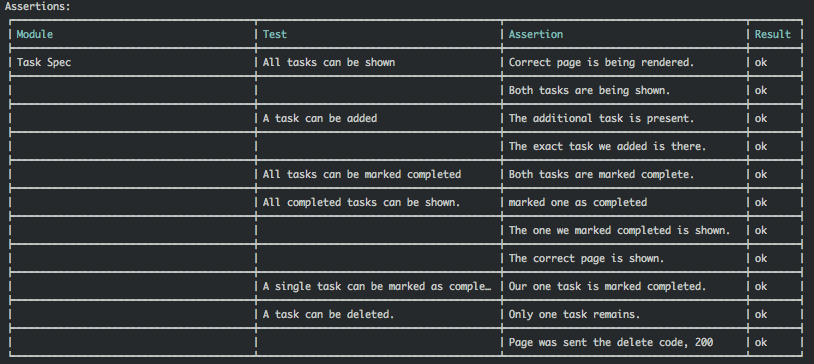
\includegraphics[width=\linewidth]{qunitrunner.png} 
  \captionof{figure}{Each individual spec is further broken down into the assertions within it.}
\end{Figure}
An interesting feature that QUnit has that I've not seen elsewhere is the ability to specify how many assertions you expect to run in the test. This is incredibly useful for callbacks. By setting an expected number of assertions, tests can no longer fail silently just because an assertion was never run. If the QUnit test finishes and the assertion count is not what was specified, it will fail the test and let you know fewer assertions were called than expected.

QUnit isn't perfect however, QUnit tests are not grouped into suites by default and the syntax for grouping them leaves much to be desired. In order to group tests into ``modules'', as QUnit calls them, the developer writes code like the following:
\begin{lstlisting}
Qunit.module("Module A"); // All code following is grouped into Module A
test("Addition", function () {
  equal(2 + 2, 4, "Two + Two = Four");
  equal(3 + 5, 8, "Three + Five = Eight");
});
test("Subtraction", function () {
  equal(4 - 2, 2, "Four - Two = Two");
  equal(2 - 2, 0, "Two - Two = Zero");
});

// More tests....

QUnit.module("Module B");
// Tests under Module B

// ... Etc
\end{lstlisting}
It is difficult to visually see where one module starts and ends and so grouping and finding the right place to add a test can be a chore.

QUnit's handling of asynchronous tests is similar to Mocha's except instead of adding a parameter to the ``it'' function, you call the ``asyncTest'' function instead of the ``test'' function and then call ``start()'' when you finish your asynchronous tests. Example:
\begin{lstlisting}
asyncTest("Async Test", function () {
  myAsyncCall(param1, param2, function () {
    // This callback expected to run when async returns

    // Test ...
    // Test ...
    // ...
    start();
  });
});
\end{lstlisting}

\paragraph{Pros}

\paragraph{Cons}

\subsubsection{Intern}

\paragraph{Pros}

\paragraph{Cons}

\subsection{Continuous Integration Frameworks}
Continuous Integration frameworks attempt to make development easier by running specified actions, usually tests, after a change to the project. This change can be simply saving a modified file, or, more usually, an action like pushing a change to a repository.

Continuous Integration frameworks, therefore, need to be flexible in the type of project they support, customizable in their chosen environments to support differing projects, and have a simple way to connect to repositories or file systems.

\subsubsection{Jenkins \cite{Jenkins}}
Jenkins is the first of the continuous integration frameworks that I tried out. It was created by developers of a previous tool called Hudson when a dispute with Oracle led them to fork the Hudson project and rename it Jenkins. As of February 2014, the Jenkins organization has over 1,100 public repositories and 570 members. \cite{JenkinsGitHub} Jenkins has, according to their website, two main focuses: (1) building and testing software continuously and (2) monitoring executions of externally-run jobs. The first focus is the general goal for any CI framework. The second focus is of note and will be discussed after the initial evaluation. 

Jenkins is a series of web pages that you set up to run on a given server. This is what it looks like:
\begin{Figure}
  \centering
  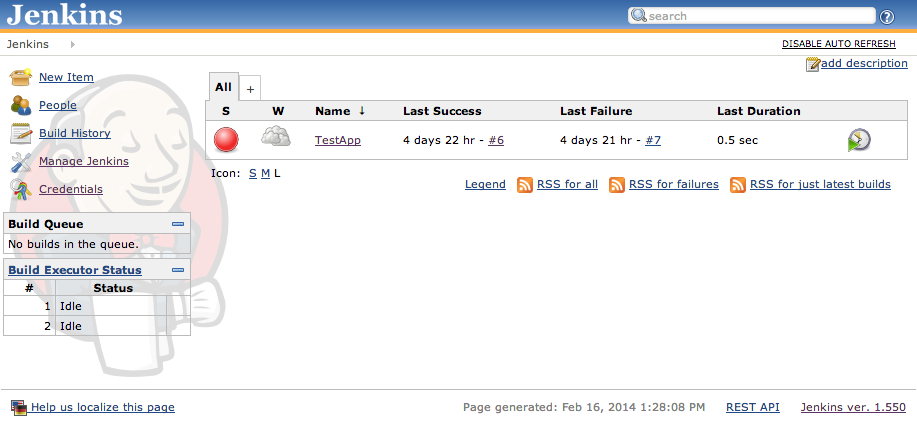
\includegraphics[width=0.95\linewidth]{jenkins.png}
\end{Figure}
Most companies give Jenkins a sub-domain on their web pages.

Jenkins comes bare-boned but is highly customizable and has a wide array of plugins. The plugins available integrate Jenkins with various services, integrate Jenkins with source control systems, and even just change the look of the Jenkins page or how it behaves. As an example, Jenkins can integrate with GitHub to run builds and tests when changes are pushed to a branch.

Because Jenkins comes bare and runs on the system of your choosing, it can run any project that you set up. The downside is that there is no support out-of-the-box unless you already have the necessary compilers, interpreters, applications, and/or libraries installed on the server running Jenkins.

One of the exceptional strengths of Jenkins is that the developer is only limited by the hardware of the machine running Jenkins. Any increase in computing power will be directly usable by Jenkins. Jenkins can run as many jobs as your server can handle at one time.

The other use for a tool like Jenkins is the ability to start services like cron jobs or similarly long-running tools and status monitors and then collect the output for them and allow the developer to check on them at any time.

Jenkins is an exceptionally strong tool for CI, but requires immense overhead in setting up the environment to run your project in. However, once the server has the necessary applications and libraries, your builds and tests will run without issue. Jenkins can run an ``unlimited'' number of builds, tests, and processes with the only limiting factor the hardware that it is running on. It is also 100\% free and can connect with public and private repositories alike.

\paragraph{Pros}

\paragraph{Cons}

\subsubsection{Travis \cite{Travis}}
Travis is an online continuous integration framework with 29 members and 64 repositories at the time of this writing. Unlike Jenkins, Travis is all online and includes a dashboard from which you can monitor your builds and processes. Travis has a free version which is fully-featured but requires your project to be open-source and a paid version which gives you more processing power and access to private repositories.

Travis requires that you projects be hosted on GitHub, but by doing so the setup is incredibly easy. You sign into Travis using your GitHub credentials and Travis pulls up all of your repositories automatically. Getting a project running with Travis is fairly easy; you create a yml file in your repository, I was able to set up everything I needed in six very simple lines.

Travis comes with incredibly thorough documentation and a wealth of built-in services like databases, notifications, deployment options, and GUI/Headless browsers. Travis supports all of the most popular databases: MySql, PostgreSql, MongoDB, CouchDB, and a myriad of others. It offers a number of notification options ranging from Email to IRC to HipChat (a chat service from Atlassian). Travis offers deployment to just about every sort of provider there is, from Heroku to AWS S3 to RubyGems and also provides the ability to create custom hooks to deploy to a provider not supported natively.

In order to get access to your private repositories, Travis offers several pricing plans, the cheapest of which is \$129 \cite{TravisPricing} for their ``Startup'' plan. That's a bit steep, but it does offer unlimited private repositories, unlimited collaborators, and two concurrent jobs. 

From what I gathered, Travis appears to be targeted at companies, not individual developers but works great if you are willing to open-source your repositories.



BREAK

Semaphore
- Public/Private doesn't matter
- 30 Day Trial, then must pay for plan
- GitHub Only
- Settings done online
- Ruby mostly, Node.js support new

Magnum (Are there ANY drawbacks... This is too good to be true)
- Public/Private doesn't matter
- Free forever as far as I can tell....?
- GitHub, BitBucket, GitLab, others too
- Auto (overridable) settings
- Too good to be true, it's in public beta right now, pricing soon.
- Xvfb support

Travis
- Free for public
- Paid for private
- GitHub only
- Requires .travis.yml file

Drone.io
- Free for public repos
- Paid for private repos
- GitHub, BitBucket, Google Code

Jenkins
- Free all the time forever because you set it up
- It'll do everything....? 
- Lots of setup


\paragraph{Pros}

\paragraph{Cons}

\subsubsection{Selenium}

\paragraph{Pros}

\paragraph{Cons}

\subsubsection{Semaphore}

\paragraph{Pros}

\paragraph{Cons}

\subsubsection{Nightwatchjs}

\paragraph{Pros}

\paragraph{Cons}

\subsection{Misc Frameworks}
\subsubsection{Sauce Labs}

\paragraph{Pros}

\paragraph{Cons}

\subsubsection{Istanbul}

\paragraph{Pros}

\paragraph{Cons}

\subsubsection{Karma}

\paragraph{Pros}

\paragraph{Cons}


\subsection{Misc Tools}
\subsection{Node Inspector}
Fantastic for debugging node.js server-side code!


%%%%%%%%%%%%%%%%%%
%%% Evaluation
%%% PX Intro
%%%	Outline test suites
%%% PX Test metrics/results
%%%%%%%%%%%%%%%%%%
\section{Evaluation}


%%%%%%%%%%%%%%%%%%%%
%%% Related Work 
%%% Similar testing frameworks
%%% 	Why they're not as good as ours
%%%%%%%%%%%%%%%%%%%%
\section{Related Work}
I was unable to find any works that attempted to bring existing technologies together to create a web testing framework. Instead, I came across a number of proprietary tools and research. For the proprietary tool an advantage of the framework I already laid out is that it is freely available and has support behind it for each individual component. There is no need to contact any paper authors to get software or support. I will, however, still outline them as they provided insight into what the problems in existing frameworks were, gaps in coverage, what was important in a framework, and inspiration and acknowledgment that this is a real problem that many people are trying to solve.

I also found research into common bugs, general testing techniques, and finding bugs that greatly improved my test cases and understanding.

\subsection{Testing Frameworks}

\subsubsection{``A Framework for Automated Testing of JavaScript Web Applications'' \cite{FrameworkForAutomatedTesting}}
A collection of IBM Researchers and two university students came up with a framework called ``Artemis'' for testing web applications. What is novel about their tool is that it generates test cases automatically based on execution patterns and feedback. They have attempted to solve the problem that writing test cases by hand is both time-consuming and often difficult. Their automatic test generation lead to an average of 69\% test coverage with enough tests generated.

Though it was an interesting and somewhat effective method, 69\% coverage is not great and this particular framework only covers the client-side, so it was incomplete for our purposes.

\subsubsection{``A Multi-Agent Software Environment for Testing Web-based Applications'' \cite{MultiAgentSoftwareEnvironment}}
Two students and a person from Lanware Limited brought AI into the web testing world with an agent-based environment for testing web applications. In order to split testing into manageable tasks for agents to carry out, they created an ontology for web testing using XML. Each agent is set up to handle one particular kind of testing with certain test data, i.e., a unit tester with data for one or two functions. This agent may then communicate with another agent who needs the results from that test, such as a test coverage agent or agent that is keeping track of test success and failure. This communication is done through a message-passing intermediary layer and a set of brokers who shuffle messages between agents.

This system is exciting and intricate but far too complex for a general web testing toolkit that just about any developer could pick up. It was important to weed techniques like this out as we wanted a fairly easy to use and understand toolkit.

\subsubsection{``A 2-Layer Model for the White-Box Testing of Web Applications'' \cite{2LayerModel}}
A couple of gentlemen at the Center for Scientific Research and Technology in Povo, Italy came with a model for white-box testing of web applications. (White box testing is when you access to the underlying code.) This paper breaks up the testing process into two abstraction levels, the navigation model, the way in which a webpage goes from page to page, and the control flow model, the way in which information is passed and stored on a given page or between pages. These constitute the 2-layers in the title. The navigation model represents high-level test cases, like asserting that a given link redirects to the correct location, while control flow represents low-level test cases, like making sure data is persisted between pages. 

This 2-layer approach is interesting and provided me with some insight, but the system was made for PHP applications and I wasn't looking to implement a brand-new system and test PolyXpress with it all in one year.

\subsubsection{``Invariant-Based Automatic Testing of AJAX User Interfaces'' \cite{InvariantBasedUseInterfaces}}
Two individuals from the SOftware Engineering Research Group at Delft University in the Netherlands came up with a way to automatically test AJAX UI. The core of this idea is using a crawler to infer a flow graph. This paper outlines an plugin for an automated tool, ATUSA, for creating state validators and test suites for covering paths discovered during crawling (with a separate tool, CRAWLJAX). Their tests show that with minimal manual effort, the use of ATUSA can lead to high code coverage and error discovery. 

This tool showed promise as an AJAX testing tool, but we wanted something more generic. Their crawler, CRAWLJAX, however, was very interesting and while we didn't use it, the techniques it used are used in other tools we have.

\subsubsection{``JSART: JavaScript Assertion-based Regression Testing'' \cite{JSART}}
Two students from the University of British Columbia created a tool called JSART that uses run-time code instrumentation and analysis to infer invariants that can be used for regression testing. When the code runs, JSART creates a number of test cases that will be run the next time the code executes. The point being to catch any discrepancies between old code and new code. They ran their tool on nine web systems with fairly strong results. The tool was not perfect and occasionally created inappropriate tests, but generally the tests were appropriate and useful.

This is a useful concept that could be integrated into the toolkit at a later time.

\subsubsection{``DOM Transactions for Testing JavaScript'' \cite{DOMTransactions}}
Three people from Albert Ludwigs University in Germany came up with a way to deal with test fixtures that are built and torn down frequently. When testing JavaScript, many of one's tests will change the underlying web page in some way. This is often different from testing traditional software where components are separated. In order to test JavaScript, test fixtures for setting up the page and tearing down the page are exceptionally important. Because these fixtures are being made and torn down frequently, this paper discusses a way to utilize transactional memory to quickly get the web page into the right state without constant setup and tear down.

This could be integrated with one of the existing tools we will use, but our goal was to collect existing tools that did not need alteration.

\subsubsection{``Testing Web Applications in Practice'' \cite{TestingInPractice}}
Four students from the University of Seville, Spain published a paper with an overview of web testing. This paper was more of an introduction to testing, outlining the concepts of “Unit Testing”, “Integration Testing”, “Regression Testing”, testing the client versus testing the server, and a few others. It also describes how to test an actual web application using PHPUnit, a library similar to JUnit, for those of you familiar with Java. When writing their tests, they suggest taking more abstract actions and breaking them up into their functional parts and testing each of those. As an example, inserting a customer into the database (albeit not that abstract) is broken into tests for the function that inserts the customer and tests for making sure the customer makes it into the database.

The paper was good refresher on testing concepts and a hands-on application of those concepts. There wasn't any new information or tools to put toward our toolkit, but it was a good reminder and outlined some testing procedures.

\subsubsection{``Contract-Driven Testing of JavaScript Code'' \cite{ContractDrivenTesting}}
Two individuals from the Albert Ludwigs University in Germany created a tool, JSConTest, that provides a framework for making contracts for a JavaScript program, allowing for guided random testing on inputs and outputs. Contracts in JSConTest are comments above each function that are of the form ``type -> type''. More complicated forms can introduce parenthesis for function types. In general, JSConTest is useful for detecting type errors on input or output based on the operations performed within a function on the input and the result being output. 

Although JSConTest could be useful in a toolkit, its source is no-where to be found and there were other, more robust, tools out there for our purposes.

\subsubsection{``JAWS: A Javascript API for the Efficient Testing and Integration of Semantic Web Services'' \cite{JAWS}}
A researcher from Ford Motor Company published a paper regarding an API, called JAWS (Javascript, AJAX, Web Service), to facilitate testing and integration of Semantic Web Services. Semantic Web Services (SWS) are the server side of machine-to-machine interaction via the internet. This is opposed to machine-to-human interaction such as web pages that you visit personally. SWS use markup that is detailed and sophisticated which conforms to certain standards but is not human-readable.

Another interesting API and project, but we are not focusing on SWS and so including a tool or API like JAWS would be overkill and beyond trying to keep the toolkit as simple and robust as possible.

\subsubsection{``WebMate: A Tool for Testing Web 2.0 Applications'' \cite{WebMate}}
Four people from Saarland University in Germany created a tool, WebMate, for automatically navigating web-pages with dynamic content and data. WebMate's goal is to output a usage model for testing purposes. This usage model allows tests to be focused on navigation as well as functionality. This dual usage leads to the ability to test the experience as well as the functions. In addition, WebMate can be used for Cross-Browser testing by running it on multiple browsers and comparing the results. In essence, WebMate is a web application crawler seeking to automatically suss out the layout and interaction between web pages to provide a model to the tester, be it a developer or the automatic testing capabilities of WebMate.

WebMate was another interesting project that could have seen use in our toolkit if crawlers weren't already available in other, more mainstream, tools.

\subsubsection{``Continuous Testing with Ruby, Rails, and JavaScript'' \cite{BookContinuousTesting}}
The well known book by Rady and Coffin talks about Continuous Testing and has lots of examples. The last two chapters of the book, six and seven, talk about setting up a Continuous Testing environment for JavaScript using Node.js and a number of other tools. It fit almost perfectly with our project and was used as the basis of my testing setup. They use JSLint for linting, Jasmine for test cases, and Watchr for running the tests continuously. Lastly it discussing writing effective tests, which is always important.

Not all of those tools made it into the eventual final toolkit, but they were all important to look at in the context of making the overarching toolkit.

\subsection{Finding Bugs}
One of the most important aspects of testing is actually finding the bugs in the program. A number of sources provided guidelines and suggestions for finding bugs in web applications.

\subsubsection{``Finding Bugs In Dynamic Web Applications'' \cite{FindingBugs}}
Seven researchers from the MIT Computer Science and Artificial Intelligence Lab wrote a paper addressing testing in dynamic web applications. Common testing techniques were not made to work with dynamic content that can be generated at the drop of a hat or click of a button. Therefore, common testing techniques are inadequate for testing dynamic web applications. This paper discusses ways to find bugs in these new-fangled dynamic web applications. They use a new technique and extended a tool called Apollo. This technique generates dynamic test cases based on concrete and symbolic execution. ``The basic idea is to execute an application on an initial input (e.g., an unconstrained or randomly chosen input), and then on additional inputs obtained by solving constraints derived from exercised control flow paths.''

Although they test PHP applications, the extension to JavaScript is fairly straightforward. We didn't use Apollo, but the techniques described within allowed for more focused and productive testing.

\subsubsection{``Testing Web Services: A Survey'' \cite{TestingWebServicesSurvey}}
Three researchers at the Centre for Research on Evolution, Search \& Testing at King's College in London wrote a survey of web frameworks for testing web services. Their focus is on Service-Oriented Computing, a paradigm in which web sites or applications provide small pieces of functionality usable by ``anyone''. These services are then combined to create more fully featured applications. What they note in particular is that when using web services, you rarely have access to the source code and must therefore black-box test them. Corollary to that is that you have to implicitly trust whoever made the service. They go through and discuss a number of frameworks and come to the conclusion that it's most certainly not a solved problem for the following reasons: The frequency of testing required, Testing without disrupting the operation of the service, Determining when testing is required and which operations need to be tested. Regarding the frequency of testing, web services often change in effort to make improvements, but those improvements can change the services and break tests. Testing without disrupting service is difficult because these services often limit accesses or simultaneous access of both a test and a running web application. Finally, determining when and what to test comes back to the trust issue. Some services provide their own testing metrics that include code coverage, number of tests, etc. But you have to trust that they are thoroughly testing whatever it may be.

\subsubsection{``A Framework for Testing RESTful Web Services'' \cite{RESTfulFramework}}
Two people from the University of Dakota School of Aerospace Studies outline a framework for testing RESTful web services. RESTful web services, short for Representation State Transfer, are, in the context of web applications, a name for web APIs that conform to a set of constraints. In particular they must offer four request methods: GET, POST, PUT, and DELETE. These methods generally connect to a database or other storage system in order to store, retrieve, or delete entries therein.

\todo{Finish reading this paper... My bad Dr. Haungs.}

\subsection{Writing Effective Test Cases}
Although not too distinct from \emph{finding bugs}, writing effective test cases is its own art form. The important of writing concise, correct, productive test cases cannot be overstated. The difference between writing one test case that effective tests multiple things and writing a single test case for every little detail is the difference between developers wanting to write tests at all and skipping it due to time constraints or frustration.

\subsubsection{``Going Faster: Testing The Web Application'' \cite{GoingFaster}}
Two employees of Evant Software wrote an article for IEEE Software regarding the testing of web applications. Mostly this paper was an overview and implementation of Test Driven Development (TDD) and eXtreme Programming, but in the middle of the article was a good section about the difficulties of testing the web and how to deal them. A few of the remarks regarding the difficulty of web testing is that often the client-side and server-side portions of web applications are written in different languages. This wasn't an issue for our application, but is still an issue for many applications. Some of the most useful advice was: ``First, test those parts of the server-side code that are not directly concerned with being part of the Web application, without involving Web peculiarities. ... Second, test those parts of the client-side code that have no server interaction. This is typically code that contains little or no business logic. ... Third, write functional tests of a low grain in the server-side language (for example, Java or C++) that simulate the request/response Web environment. ... Using this framework you can write walk-through tests that simulate the user moving through the UI''.

This step-by-step walkthrough of how to test was an excellent starting point to look at different tools and how they handled this issue.

%%%%%%%%%%%%%%%%%%
%%% Conclusion 
%%% Summary of what they just read
%%% Recap results
%%%%%%%%%%%%%%%%%%
\section{Conclusion}


%%%%%%%%%%%%%%%%%%%
%%% Future Work 
%%% Anything we wanted to do but didn't have time to
%%%%%%%%%%%%%%%%%%%
\section{Future Work}


%%%%%%%%%%%%%%%%%
%%% Appendices
%%% Actual Test Code
%%% Anything that needs an appendix
%%%%%%%%%%%%%%%%%
\section{Appendices}

% \end{multicols}
\newpage

\bibliographystyle{IEEEannot}

\bibliography{paper}

\nocite{*}

\end{document}
